\section{System Architecture}
The architecture of the proposed Search and Rescue robot is founded on the principle of mission-specific modularity. The primary objective of this design is to create a platform where both hardware and software can be adapted for different operational environments, such as collapsed buildings or open-field disaster sites, while maintaining reasonable costs. This approach allows a rescue team to augment a core robotic platform with specialized capabilities as needed.

Our methodology leverages a standard, commercially available robotic base—the Robotis TurtleBot—which provides robust and reliable locomotion. The TurtleBot chassis features a grid of pre-drilled mounting holes, which serves as the physical interface for our modular "building block" concept. New functional modules are physically attached to the chassis using a simple and direct screw-on system. Electronically, each module is wired directly to the main onboard processor, allowing for straightforward integration of custom components into the main system.

\subsection{Hardware Implementation}
The physical prototype is constructed upon a Robotis TurtleBot3 Burger, which serves as the core platform for locomotion and control. The primary onboard computer is a Raspberry Pi 4B with 4GB of RAM. The TurtleBot's Dynamixel servos are managed by a dedicated OpenCR board, which interfaces with the Raspberry Pi.

Our modular additions are integrated directly onto this base platform. The acoustic sensing capability is provided by a standard USB clip-on microphone. To enhance directed listening and improve the signal-to-noise ratio, the microphone is mounted at the focal point of a parabolic dish, which is attached to a servo motor for orientation control. For the localization task, the robot is equipped with a dedicated ESP32 microcontroller that functions as the onboard WiFi receiver and processor for RSSI measurements.

The localization infrastructure consists of three stationary beacons, each built from a standalone ESP32 module powered by AAA batteries. These beacons are positioned around the operational area to create the necessary reference grid. The complete hardware assembly is depicted in the CAD model shown in Fig.~\ref{fig:robotCAD}. To provide a clear overview, the key hardware components are summarized in Table~\ref{tab:hardware_components}.

\begin{figure}[!b]
  \centering
  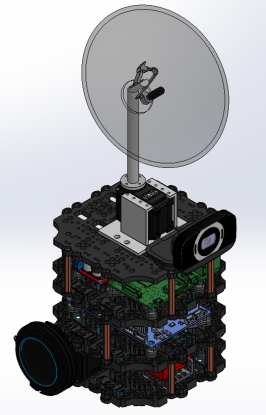
\includegraphics[width=0.65\linewidth]{robotcad.png}
  \caption{CAD model of the assembled SAR robot, showing the TurtleBot3 Burger base, onboard electronics, and sensor attachments}
  \label{fig:robotCAD}
\end{figure}

\begin{table*}[t]
  \caption{Key Hardware Components}
  \label{tab:hardware_components}
  \centering
  \begin{tabular}{lll}
    \toprule
    \textbf{Component} & \textbf{Model/Part} & \textbf{Purpose} \\
    \midrule
    Core Platform & Robotis TurtleBot3 Burger & Mobility and base structure \\
    Central Processor & Raspberry Pi 4B (4GB) & Main control, audio processing \\
    Low-level Control & OpenCR Board & Interfacing with Dynamixel servos \\
    Onboard RSSI RX & ESP32 & Dedicated WiFi RSSI processing \\
    Microphone & USB Clip-on Microphone with Parabolic Dish & Capturing ambient audio \\
    Localization Beacons & ESP32 (x3) & Stationary WiFi signal sources \\
    Power Source & TurtleBot3 Battery Pack & System power \\
    \bottomrule
  \end{tabular}
\end{table*}

\subsection{Software and Data Flow}
The robot's software architecture employs a hybrid approach, utilizing custom Python scripts for primary logic, the MQTT protocol for lightweight inter-process communication, and some elements of the Robot Operating System (ROS) for hardware interfacing. The audio classification task on the Raspberry Pi is implemented using the TensorFlow library.

The operational flow of the system is continuous and concurrent:
\begin{enumerate}
    \item \textbf{Acoustic Perception:} The main Python script on the Raspberry Pi continuously listens for audio captured by the parabolic microphone. It processes this audio stream in real-time using a TensorFlow model trained to recognize human voice patterns. The system constantly publishes the results—including the sound's orientation relative to the robot and a confidence level of human presence—to an MQTT topic.
    \item \textbf{Localization:} Concurrently, the dedicated onboard ESP32 continuously scans for WiFi signals from the three stationary beacons. Each beacon is configured to broadcast a unique and constant WiFi network name (SSID). The onboard ESP32 measures the RSSI from each beacon and uses a pre-calibrated model based on a least-squares mapping to calculate the robot's (x, y) coordinates relative to the known positions of the beacons.
    \item \textbf{Data Aggregation and Transmission:} The Raspberry Pi subscribes to the data streams from both the acoustic perception script and the ESP32 localization module. It aggregates this information—the robot's current location and the confidence/direction of any detected human voice—and transmits it to a remote operator's computer for monitoring and decision-making.
\end{enumerate}
